%!TEX root = ../booklet.tex
% ^ leave for LaTeXTools build functionality

\begin{puzzle}
  \rightImg{0.75in}{dominoRally/dominoIllustration.pdf}
  We constructed letters by tiling dominoes in a $5\times5$ square, and we
  used them to write a clue to the location of an EXTRA Puzzle.

  Unfortunately, a few extra letters have been snuck in, so you'll
  probably want to remove those first... Report your solution to
  Game HQ and earn \(100\) points!

\begin{center}
  \includegraphics[width=0.12\linewidth]{dominoRally/letterI.pdf}\hspace{0.03\linewidth}
  \includegraphics[width=0.12\linewidth]{dominoRally/letterCFake.pdf}\hspace{0.03\linewidth}
  \includegraphics[width=0.12\linewidth]{dominoRally/letterUFake.pdf}\hspace{0.03\linewidth}
  \includegraphics[width=0.12\linewidth]{dominoRally/letterT.pdf}\hspace{0.03\linewidth}
  \includegraphics[width=0.12\linewidth]{dominoRally/letterNFake.pdf}\hspace{0.03\linewidth}
  \includegraphics[width=0.12\linewidth]{dominoRally/letterS.pdf}\hspace{0.03\linewidth}
\end{center}
\begin{center}
  \includegraphics[width=0.12\linewidth]{dominoRally/letterJFake.pdf}\hspace{0.03\linewidth}
  \includegraphics[width=0.12\linewidth]{dominoRally/letterEFake.pdf}\hspace{0.03\linewidth}
  \includegraphics[width=0.12\linewidth]{dominoRally/letterF.pdf}\hspace{0.03\linewidth}
  \includegraphics[width=0.12\linewidth]{dominoRally/letterFFake.pdf}\hspace{0.03\linewidth}
  \includegraphics[width=0.12\linewidth]{dominoRally/letterGFake.pdf}\hspace{0.03\linewidth}
  \includegraphics[width=0.12\linewidth]{dominoRally/letterE.pdf}\hspace{0.03\linewidth}
\end{center}
\begin{center}
  \includegraphics[width=0.12\linewidth]{dominoRally/letterSFake.pdf}\hspace{0.03\linewidth}
  \includegraphics[width=0.12\linewidth]{dominoRally/letterHFake.pdf}\hspace{0.03\linewidth}
  \includegraphics[width=0.12\linewidth]{dominoRally/letterA.pdf}\hspace{0.03\linewidth}
  \includegraphics[width=0.12\linewidth]{dominoRally/letterQFake.pdf}\hspace{0.03\linewidth}
  \includegraphics[width=0.12\linewidth]{dominoRally/letterAFake.pdf}\hspace{0.03\linewidth}
  \includegraphics[width=0.12\linewidth]{dominoRally/letterT.pdf}\hspace{0.03\linewidth}
\end{center}
\begin{center}
  \includegraphics[width=0.12\linewidth]{dominoRally/letterOFake.pdf}\hspace{0.03\linewidth}
  \includegraphics[width=0.12\linewidth]{dominoRally/letterCFake.pdf}\hspace{0.03\linewidth}
  \includegraphics[width=0.12\linewidth]{dominoRally/letterU.pdf}\hspace{0.03\linewidth}
  \includegraphics[width=0.12\linewidth]{dominoRally/letterLFake.pdf}\hspace{0.03\linewidth}
  \includegraphics[width=0.12\linewidth]{dominoRally/letterR.pdf}\hspace{0.03\linewidth}
  \includegraphics[width=0.12\linewidth]{dominoRally/letterFFake.pdf}\hspace{0.03\linewidth}
\end{center}
\begin{center}
  \includegraphics[width=0.12\linewidth]{dominoRally/letterE.pdf}\hspace{0.03\linewidth}
  \includegraphics[width=0.12\linewidth]{dominoRally/letterDFake.pdf}\hspace{0.03\linewidth}
  \includegraphics[width=0.12\linewidth]{dominoRally/letterMFake.pdf}\hspace{0.03\linewidth}
  \includegraphics[width=0.12\linewidth]{dominoRally/letterD.pdf}\hspace{0.03\linewidth}
  \includegraphics[width=0.12\linewidth]{dominoRally/letterLFake.pdf}\hspace{0.03\linewidth}
  \includegraphics[width=0.12\linewidth]{dominoRally/letterE.pdf}\hspace{0.03\linewidth}
\end{center}
\begin{center}
  \includegraphics[width=0.12\linewidth]{dominoRally/letterWFake.pdf}\hspace{0.03\linewidth}
  \includegraphics[width=0.12\linewidth]{dominoRally/letterX.pdf}\hspace{0.03\linewidth}
  \includegraphics[width=0.12\linewidth]{dominoRally/letterDFake.pdf}\hspace{0.03\linewidth}
  \includegraphics[width=0.12\linewidth]{dominoRally/letterIFake.pdf}\hspace{0.03\linewidth}
  \includegraphics[width=0.12\linewidth]{dominoRally/letterH.pdf}\hspace{0.03\linewidth}
  \includegraphics[width=0.12\linewidth]{dominoRally/letterIFake.pdf}\hspace{0.03\linewidth}
\end{center}
\begin{center}
  \includegraphics[width=0.12\linewidth]{dominoRally/letterI.pdf}\hspace{0.03\linewidth}
  \includegraphics[width=0.12\linewidth]{dominoRally/letterJFake.pdf}\hspace{0.03\linewidth}
  \includegraphics[width=0.12\linewidth]{dominoRally/letterWFake.pdf}\hspace{0.03\linewidth}
  \includegraphics[width=0.12\linewidth]{dominoRally/letterB.pdf}\hspace{0.03\linewidth}
  \includegraphics[width=0.12\linewidth]{dominoRally/letterDFake.pdf}\hspace{0.03\linewidth}
  \includegraphics[width=0.12\linewidth]{dominoRally/letterI.pdf}\hspace{0.03\linewidth}
\end{center}
\begin{center}
  \includegraphics[width=0.12\linewidth]{dominoRally/letterSFake.pdf}\hspace{0.03\linewidth}
  \includegraphics[width=0.12\linewidth]{dominoRally/letterT.pdf}\hspace{0.03\linewidth}
  \includegraphics[width=0.12\linewidth]{dominoRally/letterRFake.pdf}\hspace{0.03\linewidth}
  \includegraphics[width=0.12\linewidth]{dominoRally/letterCFake.pdf}\hspace{0.03\linewidth}
  \includegraphics[width=0.12\linewidth]{dominoRally/letterH.pdf}\hspace{0.03\linewidth}
  \includegraphics[width=0.12\linewidth]{dominoRally/letterPFake.pdf}\hspace{0.03\linewidth}
\end{center}
\begin{center}
  \includegraphics[width=0.12\linewidth]{dominoRally/letterKFake.pdf}\hspace{0.03\linewidth}
  \includegraphics[width=0.12\linewidth]{dominoRally/letterA.pdf}\hspace{0.03\linewidth}
  \includegraphics[width=0.12\linewidth]{dominoRally/letterCFake.pdf}\hspace{0.03\linewidth}
  \includegraphics[width=0.12\linewidth]{dominoRally/letterS.pdf}\hspace{0.03\linewidth}
  \includegraphics[width=0.12\linewidth]{dominoRally/letterMFake.pdf}\hspace{0.03\linewidth}
  \includegraphics[width=0.12\linewidth]{dominoRally/letterP.pdf}\hspace{0.03\linewidth}
\end{center}
\begin{center}
  \includegraphics[width=0.12\linewidth]{dominoRally/letterQFake.pdf}\hspace{0.03\linewidth}
  \includegraphics[width=0.12\linewidth]{dominoRally/letterL.pdf}\hspace{0.03\linewidth}
  \includegraphics[width=0.12\linewidth]{dominoRally/letterJFake.pdf}\hspace{0.03\linewidth}
  \includegraphics[width=0.12\linewidth]{dominoRally/letterMFake.pdf}\hspace{0.03\linewidth}
  \includegraphics[width=0.12\linewidth]{dominoRally/letterA.pdf}\hspace{0.03\linewidth}
  \includegraphics[width=0.12\linewidth]{dominoRally/letterCFake.pdf}\hspace{0.03\linewidth}
\end{center}
\begin{center}
  \includegraphics[width=0.12\linewidth]{dominoRally/letterWFake.pdf}\hspace{0.03\linewidth}
  \includegraphics[width=0.12\linewidth]{dominoRally/letterT.pdf}\hspace{0.03\linewidth}
  \includegraphics[width=0.12\linewidth]{dominoRally/letterAFake.pdf}\hspace{0.03\linewidth}
  \includegraphics[width=0.12\linewidth]{dominoRally/letterCFake.pdf}\hspace{0.03\linewidth}
  \includegraphics[width=0.12\linewidth]{dominoRally/letterE.pdf}\hspace{0.03\linewidth}
  \includegraphics[width=0.12\linewidth]{dominoRally/letterCFake.pdf}\hspace{0.03\linewidth}
\end{center}
\begin{center}
  \includegraphics[width=0.12\linewidth]{dominoRally/letterS.pdf}\hspace{0.03\linewidth}
  \includegraphics[width=0.12\linewidth]{dominoRally/letterXFake.pdf}\hspace{0.03\linewidth}
  \includegraphics[width=0.12\linewidth]{dominoRally/letterLFake.pdf}\hspace{0.03\linewidth}
  \includegraphics[width=0.12\linewidth]{dominoRally/letterA.pdf}\hspace{0.03\linewidth}
  \includegraphics[width=0.12\linewidth]{dominoRally/letterYFake.pdf}\hspace{0.03\linewidth}
  \includegraphics[width=0.12\linewidth]{dominoRally/letterN.pdf}\hspace{0.03\linewidth}
\end{center}
\begin{center}
  \includegraphics[width=0.12\linewidth]{dominoRally/letterEFake.pdf}\hspace{0.03\linewidth}
  \includegraphics[width=0.12\linewidth]{dominoRally/letterD.pdf}\hspace{0.03\linewidth}
  \includegraphics[width=0.12\linewidth]{dominoRally/letterYFake.pdf}\hspace{0.03\linewidth}
  \includegraphics[width=0.12\linewidth]{dominoRally/letterB.pdf}\hspace{0.03\linewidth}
  \includegraphics[width=0.12\linewidth]{dominoRally/letterEFake.pdf}\hspace{0.03\linewidth}
  \includegraphics[width=0.12\linewidth]{dominoRally/letterKFake.pdf}\hspace{0.03\linewidth}
\end{center}
\begin{center}
  \includegraphics[width=0.12\linewidth]{dominoRally/letterO.pdf}\hspace{0.03\linewidth}
  \includegraphics[width=0.12\linewidth]{dominoRally/letterYFake.pdf}\hspace{0.03\linewidth}
  \includegraphics[width=0.12\linewidth]{dominoRally/letterQFake.pdf}\hspace{0.03\linewidth}
  \includegraphics[width=0.12\linewidth]{dominoRally/letterW.pdf}\hspace{0.03\linewidth}
  \includegraphics[width=0.12\linewidth]{dominoRally/letterKFake.pdf}\hspace{0.03\linewidth}
  \includegraphics[width=0.12\linewidth]{dominoRally/letterL.pdf}\hspace{0.03\linewidth}
\end{center}
\begin{center}
  \includegraphics[width=0.12\linewidth]{dominoRally/letterTFake.pdf}\hspace{0.03\linewidth}
  \includegraphics[width=0.12\linewidth]{dominoRally/letterS.pdf}\hspace{0.03\linewidth}
  \includegraphics[width=0.12\linewidth]{dominoRally/letterUFake.pdf}\hspace{0.03\linewidth}
\end{center}

\end{puzzle}

\begin{extraPuzzle}
Set `em up and knock `em down!

In the fifties, Prof. Solomon W. Golomb defined a \textbf{pent}omino to be made
up of five consecutive squares, rather than the two which make up a
domino. Two pentominos
are unique if one cannot be rotated or reflected to get the other.

Find a complete tiling of the below \(10\times6\) rectangle
using exactly twelve pentominos.
We've filled in one pentomino below to get you started, and it is possible
to find \(11\) other unique pentominos which complete the rectangle.
The team(s) turning in a valid diagram to Game HQ with the most
unique pentominos today will earn \(50\) points.

  \begin{center}
  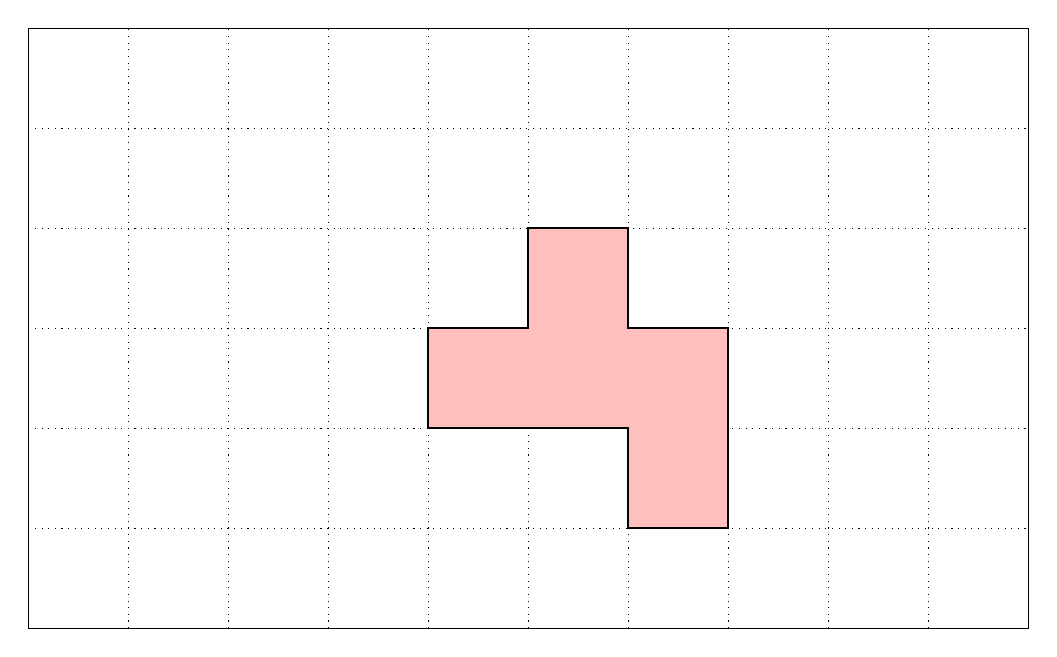
\begin{tikzpicture}
    \draw (0,0) -- (5in,0) -- (5in,3in) -- (0,3in) -- (0,0);

    \draw[dotted] (0.5in,0) -- (0.5in,3in);
    \draw[dotted] (1.0in,0) -- (1.0in,3in);
    \draw[dotted] (1.5in,0) -- (1.5in,3in);
    \draw[dotted] (2.0in,0) -- (2.0in,3in);
    \draw[dotted] (2.5in,0) -- (2.5in,3in);
    \draw[dotted] (3.0in,0) -- (3.0in,3in);
    \draw[dotted] (3.5in,0) -- (3.5in,3in);
    \draw[dotted] (4.0in,0) -- (4.0in,3in);
    \draw[dotted] (4.5in,0) -- (4.5in,3in);

    \draw[dotted] (0,0.5in) -- (5in,0.5in);
    \draw[dotted] (0,1.0in) -- (5in,1.0in);
    \draw[dotted] (0,1.5in) -- (5in,1.5in);
    \draw[dotted] (0,2.0in) -- (5in,2.0in);
    \draw[dotted] (0,2.5in) -- (5in,2.5in);

    \filldraw [thick, fill=pink]
    (2in,1in) -- (2in,1.5in) --
    (2.5in,1.5in) -- (2.5in,2in) --
    (3in,2in) -- (3in,1.5in) --
    (3.5in,1.5in) -- (3.5in,0.5in) --
    (3in,0.5in) -- (3in,1in) --
    cycle;
  \end{tikzpicture}
  \end{center}
\end{extraPuzzle}